\begin{frame}{Rete}

\begin{figure}[h!]
\centering
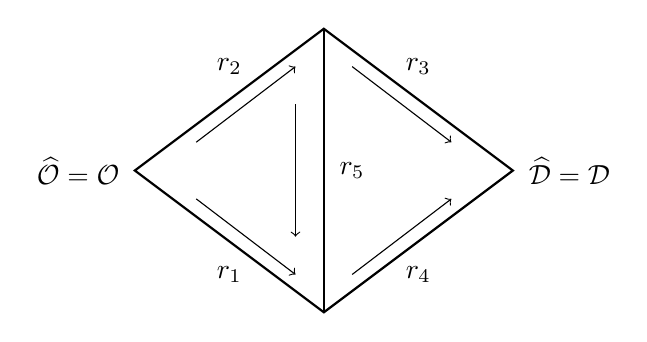
\begin{tikzpicture}[scale=1.2]

\coordinate (L) at (0,0);
\coordinate (T) at (2,1.5);
\coordinate (R) at (4,0);
\coordinate (B) at (2,-1.5);

\draw[thick] (L) -- (T) -- (R) -- (B) -- cycle;
\draw[thick] (T) -- (B);

\draw[->] (0.65,0.3) -- (1.7,1.1);

\draw[->] (0.65,-0.3) -- (1.7,-1.1);

\draw[->] (2.3,1.1) -- (3.35,0.3);

\draw[->] (2.3,-1.1) -- (3.35,-0.3);

\draw[->] (1.7, 0.7) -- (1.7, -0.7);

\node at (1,1.1) {$r_2$};
\node at (1,-1.1) {$r_1$};
\node at (3,1.1) {$r_3$};
\node at (3,-1.1) {$r_4$};
\node at (2.3, 0) {$r_5$};
\node at (-0.6, 0) {$\widehat{\mathcal{O}} = \widecheck{\mathcal{O}}$};
\node at (4.6, 0) {$\widehat{\mathcal{D}} = \widecheck{\mathcal{D}}$};
\end{tikzpicture}

\end{figure}

\end{frame}